%============================ DISEÑO ELECTRÓNICO (ENTREGA 2) =================
\chapter{Diseño electrónico y hardware}
\label{cap:electronica}

\section{Arquitectura de hardware}
El hardware de EILOR se compone de tres elementos activos ---la placa ESP32, una pantalla OLED y un pulsador--- más la alimentación. El ESP32 actúa como unidad central: integra las radios de 2.4~GHz, gobierna la pantalla por el bus I\textsuperscript{2}C y lee el pulsador por una entrada digital con resistencia \emph{pull\nobreakdash-up} interna. La Figura~\ref{fig:esquematico} presenta el diagrama de conexiones.

\begin{figure}[H]
\centering
\setlength{\fboxsep}{0pt}\setlength{\fboxrule}{0.4pt}%
\fcolorbox{gray!45}{white}{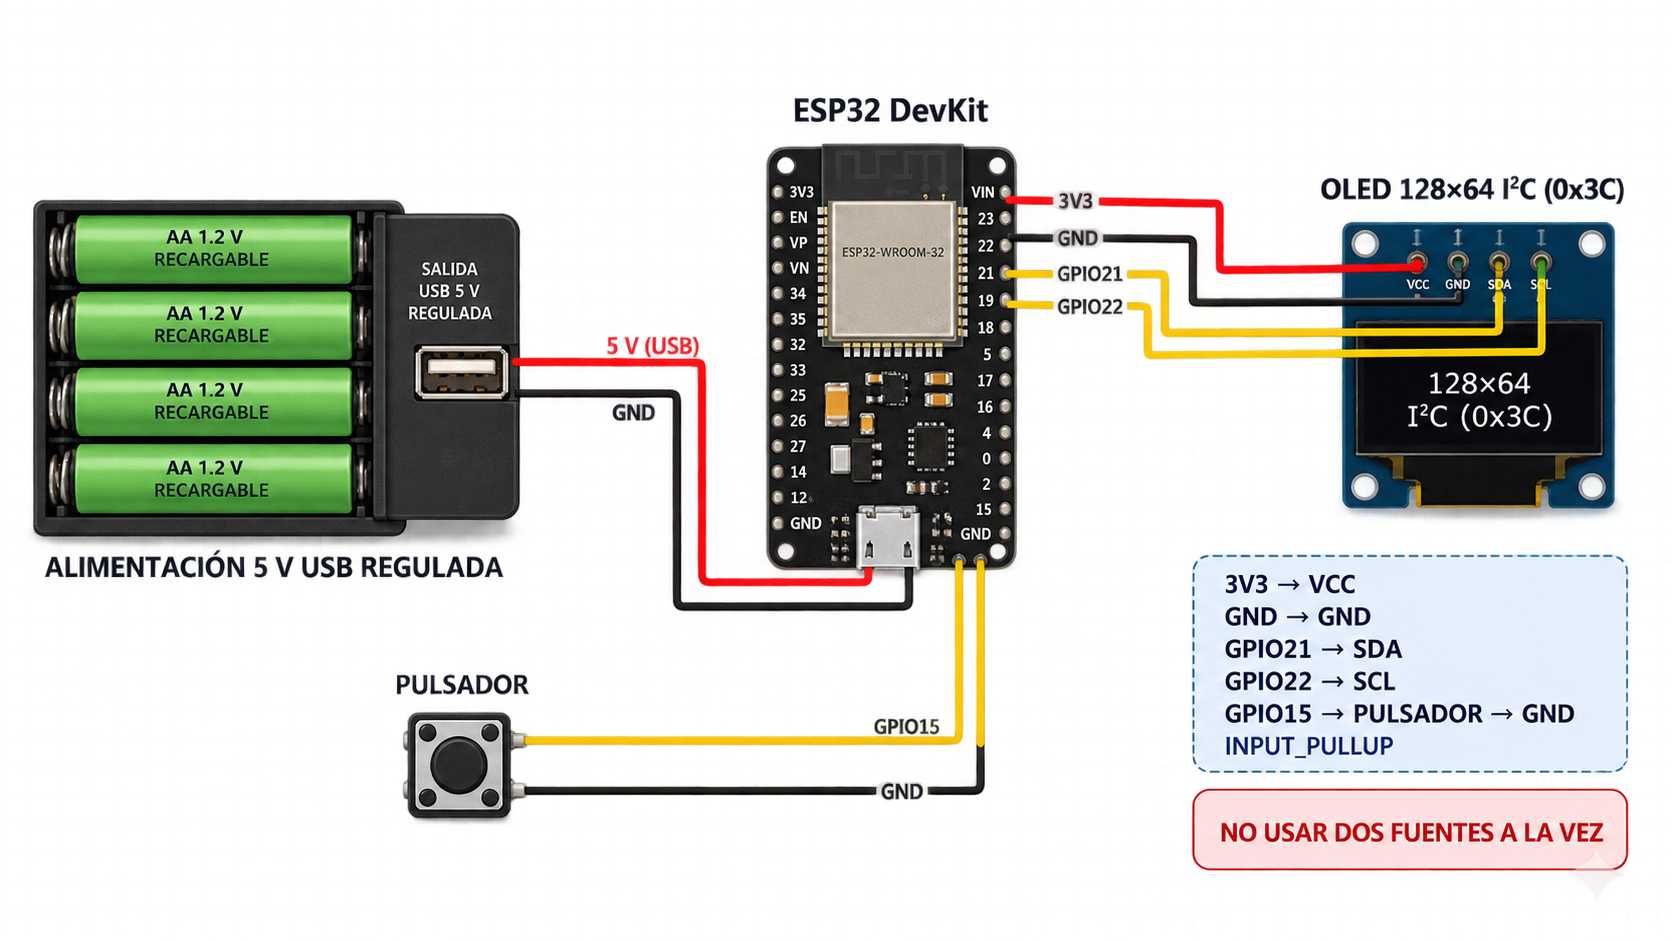
\includegraphics[width=0.98\linewidth]{figuras/diagrama-electronico-eilor}}
\caption{Diagrama funcional de conexiones y alimentación autónoma de EILOR. Los colores identifican alimentación positiva (rojo), tierra (negro) y señales (amarillo); la posición gráfica de los terminales no sustituye el pinout de la Tabla~\ref{tab:pinout}.}
\label{fig:esquematico}
\end{figure}

La figura fue generada con asistencia de inteligencia artificial y posteriormente
contrastada con el firmware del proyecto y la documentación del fabricante. La
verificación confirmó GPIO21 para SDA, GPIO22 para SCL y GPIO15 para el pulsador;
asimismo, la guía de la placa establece que USB, 5V/GND y 3V3/GND son alternativas
de alimentación mutuamente excluyentes \parencite{espressifdevkit2026}. Por ello,
debe utilizarse una sola fuente: en operación autónoma, un portapilas con salida
USB regulada a 5~V; durante programación, el USB del computador, desconectando
previamente el portapilas.

\section{Asignación de pines (pinout)}
La Tabla~\ref{tab:pinout} detalla las conexiones. El pulsador se conecta entre GPIO15 y GND; al configurarse la entrada como \code{INPUT\_PULLUP}, el pin se lee en alto en reposo y en bajo al pulsar, eliminando la necesidad de una resistencia externa.

\begin{table}[H]
\centering
\caption{Asignación de pines del ESP32}
\label{tab:pinout}
\footnotesize
\begin{tabularx}{\linewidth}{@{}l l l X@{}}
\toprule
\textbf{Pin ESP32} & \textbf{Señal} & \textbf{Componente} & \textbf{Notas} \\
\midrule
3V3 & Alimentación & OLED VCC & Lógica y alimentación a 3.3~V \\
GND & Común & OLED / Pulsador & Referencia de tierra compartida \\
GPIO21 & SDA (I\textsuperscript{2}C) & OLED & Datos del bus I\textsuperscript{2}C \\
GPIO22 & SCL (I\textsuperscript{2}C) & OLED & Reloj del bus I\textsuperscript{2}C \\
GPIO15 & Entrada digital & Pulsador & \code{INPUT\_PULLUP}; activo en bajo \\
\bottomrule
\end{tabularx}
\end{table}

\section{Lista de materiales (BOM)}
La Tabla~\ref{tab:bom} presenta la lista de materiales con un costo estimado referencial.

\begin{table}[H]
\centering
\caption{Lista de materiales y costo estimado}
\label{tab:bom}
\footnotesize
\begin{tabularx}{\linewidth}{@{}X c c c@{}}
\toprule
\textbf{Componente} & \textbf{Cant.} & \textbf{Costo unit. (USD)} & \textbf{Subtotal (USD)} \\
\midrule
Placa ESP32 DevKit (WROOM-32) & 1 & 6.50 & 6.50 \\
Pantalla OLED SSD1306 0.96" I\textsuperscript{2}C & 1 & 3.00 & 3.00 \\
Pulsador momentáneo & 1 & 0.20 & 0.20 \\
Protoboard y cables Dupont & 1 & 3.00 & 3.00 \\
Cable USB de alimentación & 1 & 1.50 & 1.50 \\
Portapilas 4\(\times\)AA con salida USB regulada a 5~V y pilas NiMH & 1 & 10.00 & 10.00 \\
\midrule
\multicolumn{3}{r}{\textbf{Total estimado}} & \textbf{24.20} \\
\bottomrule
\end{tabularx}
\end{table}

\section{Diseño conceptual de la carcasa}

La Figura~\ref{fig:carcasa-eilor} propone una carcasa de dos piezas imprimible en
3D. El diseño separa el portapilas de la electrónica, mantiene accesibles la
pantalla, el pulsador y el puerto USB, incorpora ventilación y reserva una zona
sin metal frente a la antena impresa del ESP32. Los postes de montaje y canales
internos inmovilizan las placas y reducen esfuerzos sobre los conductores.

\begin{figure}[H]
\centering
\setlength{\fboxsep}{0pt}\setlength{\fboxrule}{0.4pt}%
\fcolorbox{gray!45}{white}{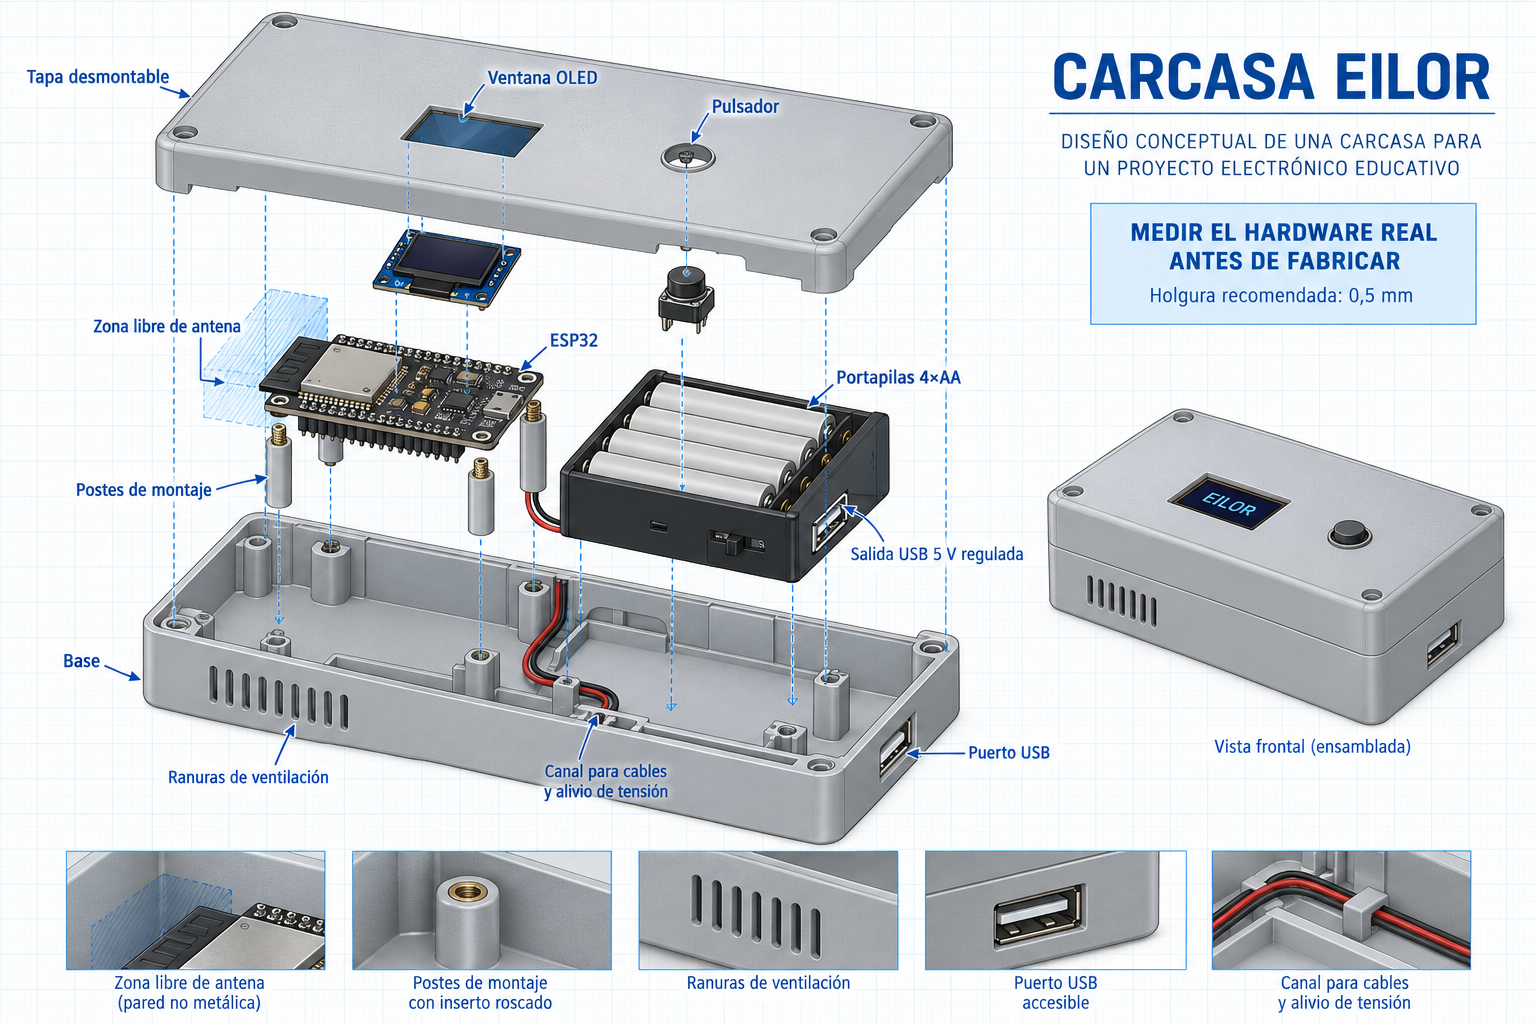
\includegraphics[width=0.98\linewidth]{figuras/carcasa-eilor-conceptual}}
\caption{Propuesta conceptual de carcasa para EILOR con compartimento de pilas, acceso a USB y zona libre frente a la antena.}
\label{fig:carcasa-eilor}
\end{figure}

La imagen de carcasa es una referencia de distribución, no un plano listo para
fabricación. Antes de modelar el archivo STL deben medirse con calibrador la placa,
la OLED, el pulsador, el portapilas y la posición exacta de conectores y orificios.
Se recomienda una holgura inicial de 0.5~mm por lado, prototipar primero la base y
confirmar que ningún poste, tornillo o cable invada la zona de la antena.

\section{Consideraciones de alimentación y coexistencia RF}
El consumo del ESP32 durante el escaneo activo con ambas radios puede presentar picos de corriente; por ello se recomienda alimentación regulada de 5~V por USB capaz de entregar al menos 500~mA. Las pilas AA no se conectan directamente a 3V3 ni a 5V: el portapilas debe integrar una salida USB regulada. En el firmware se habilita \code{WiFi.setSleep(true)} para favorecer la \emph{coexistencia} temporal entre Wi\nobreakdash-Fi y BLE, que comparten la misma radio de 2.4~GHz, evitando la inanición de una tecnología por la otra. La captura fotográfica del montaje físico se incorpora en el Anexo correspondiente.

\captura[0.85]{foto-montaje-monitor-serie}{Montaje físico del prototipo (ESP32 + OLED sobre \emph{protoboard}) y monitor serie durante la puesta en marcha.}
